\documentclass[a4paper,12pt]{article}

\usepackage{eurosym}
\usepackage{hyperref}
\usepackage{graphicx}
\usepackage{tikz}
\usepackage{circuitikz}

\graphicspath{{./immagini/}}

\title{Arduino Gameboy}
\author{Samuele Cerea e Andrea Facoetti}

\begin{document}

\maketitle
\pagenumbering{gobble} % rimuovi i numeri dalle pagine

\section{Obbiettivo}
L'obbiettivo di questo progetto \`e quello di creare una piccola console
portatile, simile al Gameboy, con un Arduino. Quindi questa console deve essere
in grado di caricare dei giochi da una cartuccia e poi eseguirli.

\section{Componenti}
\begin{center}
	\begin{tabular}{||c|c|c|c||}
		\hline
		Quantit\`a & Nome & Prezzo & Immagine \\
		\hline\hline
		1 & \href{https://www.amazon.it/dp/B01MRJR8UF}{Arduino Uno} & 15,99\euro & 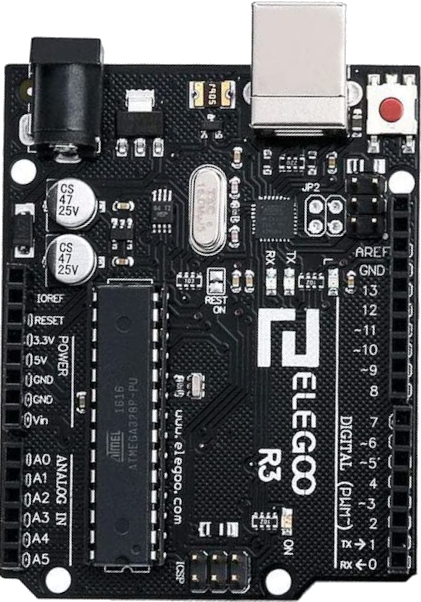
\includegraphics[width=4cm]{arduino} \\
		\hline
		1 & \href{https://www.amazon.it/dp/B07WPBQXJ9}{Kit Pulsanti} & 8,99\euro & 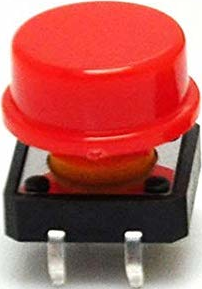
\includegraphics[width=4cm]{pulsanti} \\
		\hline
		1 & \href{https://www.amazon.it/dp/B06X1DX5WS}{Lettore Scheda SD SPI} & 5,99\euro & 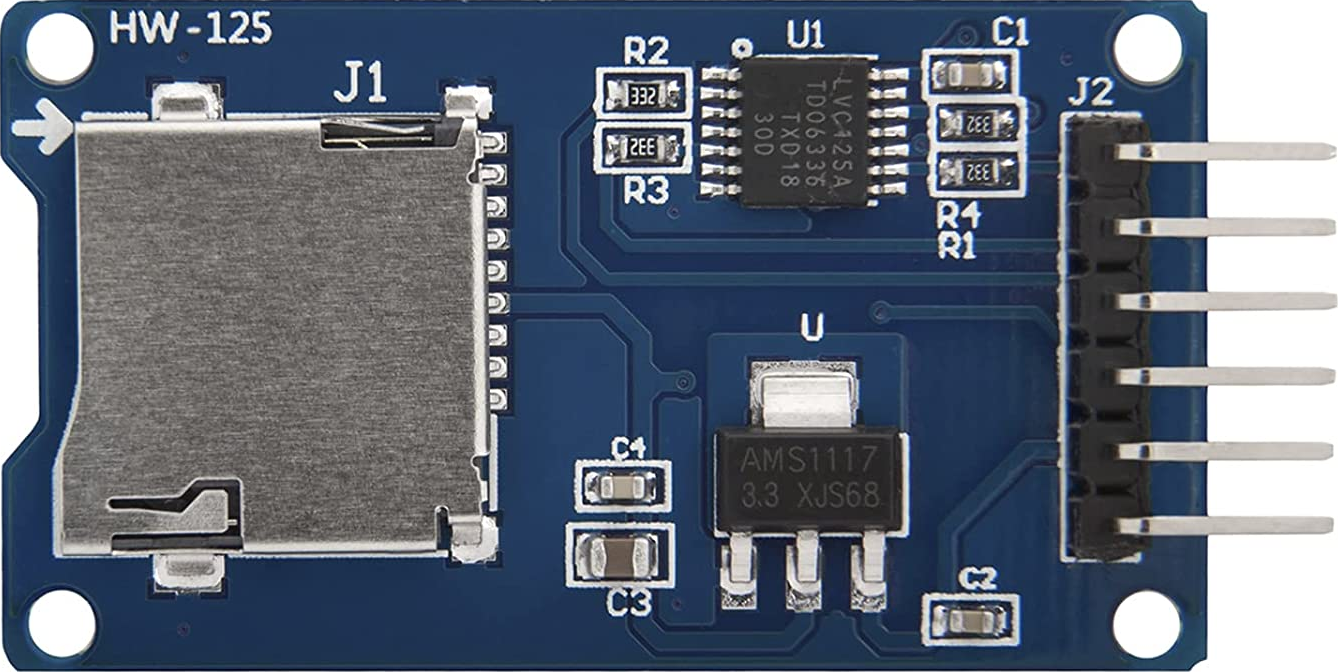
\includegraphics[width=4cm]{lettoreSD} \\
		\hline
		1 & \href{https://www.amazon.it/dp/B07G223CFP}{Display OLED 128x64 2,42 pollici SPI} & 31,99\euro & 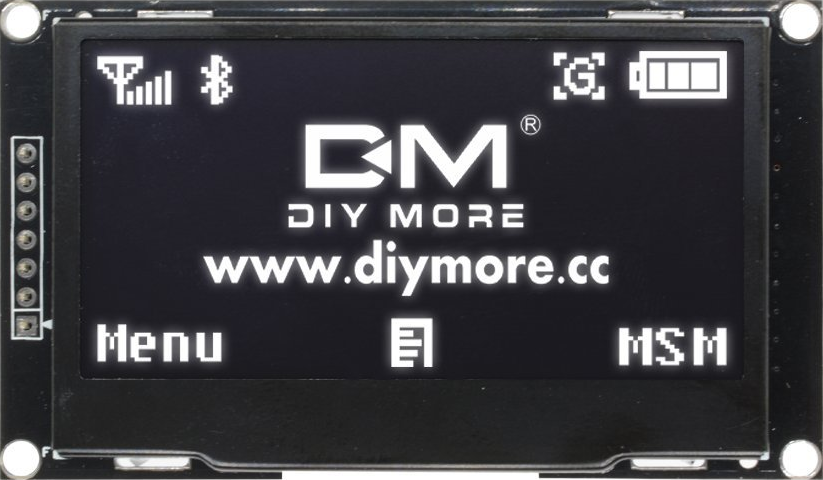
\includegraphics[width=4cm]{display} \\
		\hline
		& Cavi jumper & ~5,00\euro & \\
		\hline
		& Filo solido 22 AWG & ~10,00\euro & \\
		\hline
		3 & Breadboard & ~5,00\euro & \\
		\hline
\end{tabular}
\end{center}

\section{Circuito}
\begin{figure}[h!]
	\begin{center}
		\begin{circuitikz}
			\ctikzset{multipoles/dipchip/width=3}
			\draw (0,0) node[dipchip, num pins=26, no topmark, hide numbers, draw only pins={4-9, 14-26}](C){Arduino};
			\node [right, font=\tiny] at (C.bpin 4) {Pin A0};
			\node [right, font=\tiny] at (C.bpin 5) {Pin A1};
			\node [right, font=\tiny] at (C.bpin 6) {Pin A2};
			\node [right, font=\tiny] at (C.bpin 7) {Pin A3};
			\node [right, font=\tiny] at (C.bpin 8) {Pin A4};
			\node [right, font=\tiny] at (C.bpin 9) {Pin A5};

			\node [left, font=\tiny] at (C.bpin 26) {Pin 0};
			\node [left, font=\tiny] at (C.bpin 25) {Pin 1};
			\node [left, font=\tiny] at (C.bpin 24) {Pin 2};
			\node [left, font=\tiny] at (C.bpin 23) {Pin 3};
			\node [left, font=\tiny] at (C.bpin 22) {Pin 4};
			\node [left, font=\tiny] at (C.bpin 21) {Pin 5};
			\node [left, font=\tiny] at (C.bpin 20) {Pin 6};
			\node [left, font=\tiny] at (C.bpin 19) {Pin 7};
			\node [left, font=\tiny] at (C.bpin 18) {Pin 9};
			\node [left, font=\tiny] at (C.bpin 17) {Pin 10};
			\node [left, font=\tiny] at (C.bpin 16) {Pin 11};
			\node [left, font=\tiny] at (C.bpin 15) {Pin 12};
			\node [left, font=\tiny] at (C.bpin 14) {Pin 13};


			\draw (C.pin 4) -- ++(-2.0, 0) to [nopb] ++(-2, 0) node[ground]{};
			\draw (C.pin 5) -- ++(-.5, 0) -- ++(0, -2) -- ++(-1.5, 0) to [nopb] ++(-2, 0) node[ground]{};
			\draw (C.pin 6) -- ++(-1.0, 0) to [nopb] ++(-2, 0) node[ground]{};
			\draw (C.pin 7) -- ++(-3.5, 0) to [nopb] ++(-2, 0) node[ground]{};
		\end{circuitikz}
	\end{center}
\end{figure}

\subsection{Leggere input di un bottone}
\subsection{Il bus SPI}

\section{Codice}

\subsection{Il bootloader}
\subsubsection{Come programmere il bootloader}

\section{Limitazioni e Miglioramenti}

\section{Risorse e librerie utilizzate}

\end{document}
